\documentclass{article}
\usepackage{amsmath}
\usepackage{mathtools}
\usepackage{graphicx}
\usepackage{amssymb}
\usepackage{caption}
\usepackage{subcaption}
\usepackage{listings}
\usepackage{color}
\usepackage{hyperref}
\usepackage{placeins}
\usepackage{tikz}
\usepackage[a4paper,vmargin=3cm]{geometry}
\usepackage[linesnumbered]{algorithm2e}
\hypersetup{
    colorlinks=true,
    linkcolor=blue,
    filecolor=magenta,
    urlcolor=cyan
}
\SetKw{KwAnd}{and}
\SetKw{KwOr}{or}
\usetikzlibrary{shapes, arrows.meta, positioning, matrix, calc}

\title{Project Wetenschappelijk Rekenen}
\author{Sys, Jonas}

\begin{document}
\newcommand{\sgntxt}[2]{\stackrel{\text{#2}}{#1}}
\begin{titlepage}
 \maketitle
\end{titlepage}

\tableofcontents
\pagebreak

\section{Nulpunten van Veeltermen}
\subsection{De companionmatrix}
\subsubsection{Stelling}
\(\forall p(x): p(x)\) is een monische veelterm \(\land gr(p) = n \geq 1 \) \\
\(\implies \forall x_0 \in eigVl(C_p): p(x_0) = 0\)

\subsubsection{Bewijs}
\textbf{Inductie}: \\

\textbf{Inductiebegin}: \(n = 1\)
\begin{align*}
 p_1(x) &= x + c_0 \implies \\
 C_{p_1} &= [-c_0] \implies \\
 \rho(C_{p_1}) &= det(C_{p_1} - \lambda * I) \\
 &= -c_0 - \lambda \\
 &= (-1)^1 p_1
\end{align*}

\textbf{Inductiestap}: geldig voor graad \(n \implies\) geldig voor graad \(n + 1\) \\
Neem \(p_{n+1}(x) = x^{n+1} + \sum_{i=0}^{n}{(c_i*x^i)}\) en \(p_n(x) = x^n + \sum_{i=0}^{n-1}{(c_{i+1}*x^i)}\) (\(p_n\) zal later gebruikt worden voor inductie).
\begin{align*}
 C_{p_{n+1}} &= \begin{bmatrix}
	0 & 0 & \hdots & 0 & -c_0\\
	1 & 0 & \hdots & 0 & -c_1\\
	\vdots & \vdots & \ddots & \vdots & \vdots\\
	0 & 0 & \hdots & 0 & -c_{n-1}\\
	0 & 0 & \hdots & 1 & -c_n\\
 \end{bmatrix} \\
 &\Downarrow \text{(karakteristieke veelterm)} \\
 \rho(C_{p_{n+1}}) &= \begin{vmatrix}
	-\lambda & 0 & \hdots & 0 & -c_0\\
	1 & -\lambda & \hdots & 0 & -c_1\\
	\vdots & \vdots & \ddots & \vdots & \vdots\\
	0 & 0 & \hdots & -\lambda & -c_{n-1}\\
	0 & 0 & \hdots & 1 & -c_n-\lambda\\
 \end{vmatrix} \\
 &\Downarrow \text{(uitwerken naar eerste rij)} \\
 \rho(C_{p_{n+1}}) &= (-\lambda)* \begin{vmatrix}
	-\lambda & 0 & \hdots & 0 & -c_1\\
	1 & -\lambda & \hdots & 0 & -c_2\\
	\vdots & \vdots & \ddots & \vdots & \vdots\\
	0 & 0 & \hdots & -\lambda & -c_{n-1}\\
    0 & 0 & \hdots & 1 & -c_{n-1} - \lambda\\
 \end{vmatrix} + (-1)^n * (-c_0) * \begin{vmatrix}
	1 & -\lambda & \hdots & 0 & 0\\
	0 & 1 & \hdots & 0 & 0\\
	\vdots & \vdots & \ddots & \vdots & \vdots\\
    0 & 0 & \hdots & 1 & -\lambda\\
	0 & 0 & \hdots & 0 & 1\\
 \end{vmatrix} \\
 &= (-1)^n * \rho(C_{p_n}) + (-1)^{n+1} * c_0 \\
 &= (-1)^n * (-\lambda) * \left(\lambda^n + \sum_{i=0}^{n-1}{(c_{i+1}*\lambda^i)}\right) + (-1)^{n+1} * c_0 \\
 &= (-1)^{n+1} * \left(\lambda^{n+1} + \sum_{i=0}^{n-1}{(c_{i+1}*\lambda^{i+1})}\right) + (-1)^{n+1} * c_0 \\
 &= (-1)^{n+1} * \left(\lambda^{n+1} + \sum_{i=0}^{n}{(c_i * \lambda^i)}\right) \\
 &= (-1)^{n+1} * p_{n+1}(\lambda)
\end{align*}
Aangezien de karakteristieke veelterm van de companionmatrix en de originele veelterm (desnoods op een teken na) aan elkaar gelijk zijn, zijn de wortels van beiden ook gelijk. Aangezien de wortels van de karakteristieke veelterm van de companionmatrix de eigenwaarden zijn, geldt het te bewijzen.

\subsubsection{Sage-algoritme}
De algoritmen voor deze opgave werden getest door middel van de testcode in appendix A.


\textbf{Een eerste nai\"eve implementatie:} op basis van het idee dat de nulwaarden van een veelterm niet veranderen wanneer we een veelterm vermenigvuldigen met een getal \(c \in I\!R_0\). Hiermee kunnen wel elke veelterm \(p_n\) monisch maken door \(p'_n(x) = \frac{p_n(x)}{c_n}\) te gebruiken (\(c_n\) is de hoogstegraadco\"effici\"ent van \(p_n\)).
\begin{lstlisting}[language=Python]
def companion_solve(poly):
    for i in poly:
        div = i
    mat = companion_matrix(poly / div)
    solutions = mat.eigenvalues()
    return solutions
\end{lstlisting}
Deze implementatie heeft nog een paar probleempjes: bij het berekenen van \verb|poly / div| kunnen afrondingsfouten ontstaan (waardoor de companionmatrix niet meer berekend kan worden). Daardoor wordt een groot aantal van de testen overgeslagen. Daarnaast zitten er blijkbaar nog afrondingsfouten bij de berekening zelf, zoals te zien in de resultaten van de testen (voor elke graad, 10.000 testen gerund, met tolerantie \verb|1e-10|):\\
\begin{tabular}{|c|c|c|c|}
 \hline
 \textbf{Graad veelterm} & \textbf{Overgeslagen} & \textbf{Fouten} & \textbf{Slaagpercentage} \\
 \hline
 2  & 1517 & 0   & 84.83\% (100.0\%) \\
 3  & 1582 & 3   & 84.15\% (99.96\%) \\
 4  & 1555 & 24  & 84.21\% (99.72\%) \\
 5  & 1556 & 115 & 83.29\% (98.64\%) \\
 6  & 1563 & 255 & 81.82\% (96.98\%) \\
 7  & 1537 & 388 & 80.75\% (95.42\%) \\
 8  & 1533 & 579 & 78.88\% (93.16\%) \\
 9  & 1567 & 772 & 76.61\% (90.85\%) \\
 10 & 1506 & 890 & 76.04\% (89.52\%) \\
 \hline
\end{tabular} \\
Waarbij de slaagpercentages als volgt uitgerekend worden: \(proc = \frac{aantal - overgeslagen - fout}{aantal}\) en tussen haakjes \(proc' = \frac{aantal - overgeslagen - fout}{aantal - overgeslagen}\). Een manier om het foutpercentage te verminderen, is het gebruik van \verb|RealField(100)| in de plaats van \verb|RDF|. Dit vertraagt het volledige proces, natuurlijk. Het aantal overgeslagen testen verminderd helaas niet hiermee (tolerantie \verb|1e-15|):\\
\begin{tabular}{|c|c|c|c|}
 \hline
 \textbf{Graad veelterm} & \textbf{Overgeslagen} & \textbf{Fouten} & \textbf{Slaagpercentage} \\
 \hline
 2  & 1601 & 0   & 83.99\% (100.0\%) \\
 3  & 1534 & 0   & 84.66\% (100.0\%) \\
 4  & 1510 & 0   & 84.90\% (100.0\%) \\
 5  & 1486 & 0   & 85.14\% (100.0\%) \\
 6  & 1502 & 2   & 85.15\% (100.0\%) \\
 7  & 1462 & 1   & 84.96\% (99.98\%) \\
 8  & 1511 & 7   & 84.82\% (99.92\%) \\
 9  & 1562 & 6   & 84.32\% (99.93\%) \\
 10 & 1535 & 23  & 84.42\% (99.73\%) \\
 \hline
\end{tabular} \\
Het valt op dat het aantal veeltermen dat overgeslagen werd, ongeveer gelijk blijft.

\textbf{Het overslaan vermijden:} Nu worden er een zeer groot deel van de veeltermen overgeslagen door afrondingsfouten. Dit kunnen we vermijden door na de deling de co\"effic\"ent bij de grootste macht van \(x\) standaard op \(1\) te zetten. Dit klopt omdat deze co\"effici\"ent altijd door zichzelf gedeeld wordt, en het resultaat van \(\frac{n}{n}\) per definitie gelijk is aan \(1\). Deze aanpak resulteert in de volgende code:
\begin{lstlisting}[language=Python]
def companion_solve(poly, ring=RDF):
    tring.<x> = ring[]
    c = (poly / poly.coefficients()[-1]).coefficients()
    c[-1] = 1
    poly2 = tring(c)
    mat = companion_matrix(poly2)
    solutions = mat.eigenvalues()
    return solutions
\end{lstlisting}
Zoals verwacht worden er nu geen veeltermen meer overgeslagen:\\
\begin{tabular}{|c|c|c|c|}
 \hline
 \textbf{Graad veelterm} & \textbf{Overgeslagen} & \textbf{Fouten} & \textbf{Slaagpercentage} \\
 \hline
 2  & 0 & 0    & 100.0\% (100.0\%) \\
 3  & 0 & 3    & 99.97\% (99.97\%) \\
 4  & 0 & 45   & 99.55\% (99.55\%) \\
 5  & 0 & 158  & 98.42\% (98.42\%) \\
 6  & 0 & 287  & 97.13\% (97.13\%) \\
 7  & 0 & 429  & 95.71\% (95.71\%) \\
 8  & 0 & 647  & 93.53\% (93.53\%) \\
 9  & 0 & 887  & 91.13\% (91.13\%) \\
 10 & 0 & 1111 & 88.89\% (88.89\%) \\
 \hline
\end{tabular} \\
Als we bij het eerste algoritme de overgeslagen testen overlaten, krijgen we een gelijkaardige trend voor het percentage correcte testen. Door het wegwerken van de afrondingsfout bij de hoogstegraadseenterm, elimineren we een groot deel van de fouten (de overgeslagen testen, die anders mislukken). Natuurlijk zorgt ook hier voor een groter aantal bits (\verb|RealField(100)|) voor een lager foutenpercentage (maar het opschalen van de precisie zorgt ook voor een veel tragere uitvoering):\\
\begin{tabular}{|c|c|c|c|}
 \hline
 \textbf{Graad veelterm} & \textbf{Overgeslagen} & \textbf{Fouten} & \textbf{Slaagpercentage} \\
 \hline
 2  & 0 & 0    & 100.0\% (100.0\%) \\
 3  & 0 & 0    & 100.0\% (100.0\%) \\
 4  & 0 & 0    & 100.0\% (100.0\%) \\
 5  & 0 & 1    & 99.99\% (99.99\%) \\
 6  & 0 & 4    & 99.96\% (99.96\%) \\
 7  & 0 & 15   & 99.85\% (99.85\%) \\
 8  & 0 & 40   & 99.60\% (99.60\%) \\
 9  & 0 & 58   & 99.42\% (99.42\%) \\
 10 & 0 & 92   & 99.08\% (99.08\%) \\
 \hline
\end{tabular} \\
Opvallend is dat bij deze aanpak het aantal foute, niet-overgeslagen testen merkbaar groter is dan bij de versie zonder de co\"effici\"entencorrectie.
Hieronder een grafische vergelijking tussen de algoritmen:
\begin{figure}[!htb]
 \caption{Vergelijking algortimen}
 \begin{subfigure}{0.49\textwidth}
   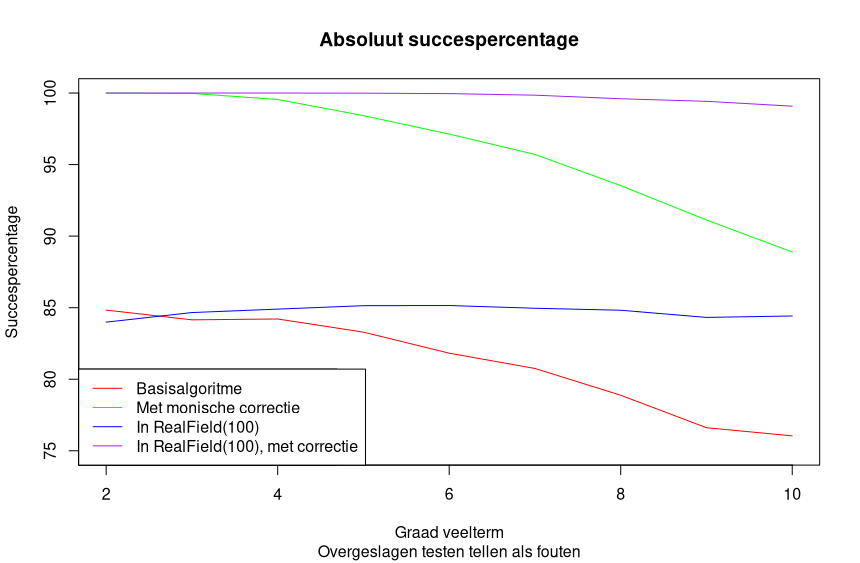
\includegraphics[width=0.9\textwidth]{figures/plot_abs}
 \end{subfigure}
 \begin{subfigure}{0.49\textwidth}
  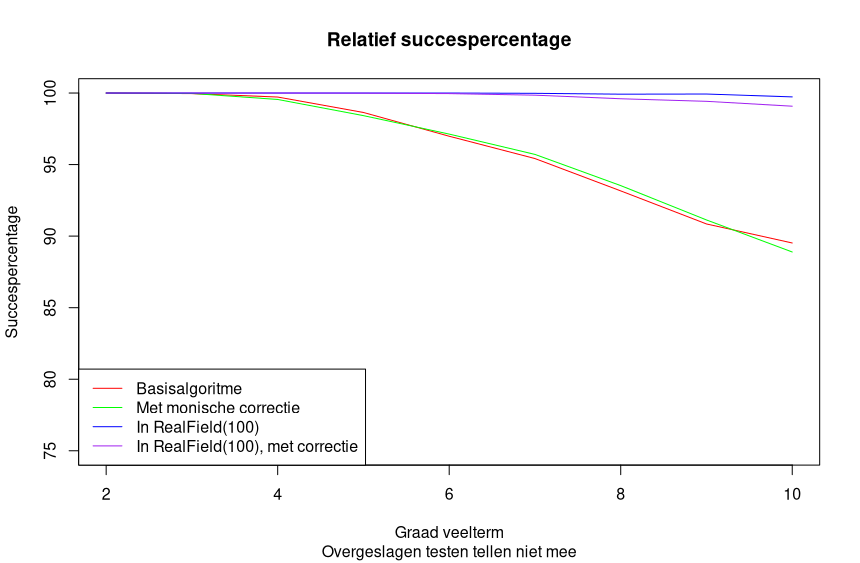
\includegraphics[width=0.95\textwidth]{figures/plot_rel}
 \end{subfigure}
\end{figure}

\subsection{Methode van Durand-Kerner}
\textbf{Een eerste na\"ieve implementatie:} door middel van de code voor de companionmatrix maken we eerst opnieuw de veelterm monisch, waarna we onderstaande berekening een aantal keer overlopen (bepaald door de parameter \verb|iterations|).
\[
 x^{(n+1)}_i = x^{(n)}_i - \frac{p\left(x^{(n)}_i\right)}{\prod_{j \neq i}{\left(x^{(n)}_i - x^{(n)}_j\right)}}
\]
Figuur 2 bevat de resultaten voor twee (re\"eele) veeltermen. Een opvallend resultaat is dat het algoritme de nulwaarde 0 nooit vindt (ook niet bij complexe veeltermen). Voor testen met de (complexe) veeltermen (\(x^3 - x^2 + (-5 + 2i)x + (-3 - 6i)\)) en (\(x^2 - (3+2i)x - (1 - 3i)\)) zijn de resultaten erg gelijkaardig: snelle, lokale convergentie.
\begin{figure}[!htb]
 \caption{Resultaten}
 \begin{subfigure}{0.49\textwidth}
  \caption{\(2x^4 + 14x^3 + 14x^2 - 30x\)}
  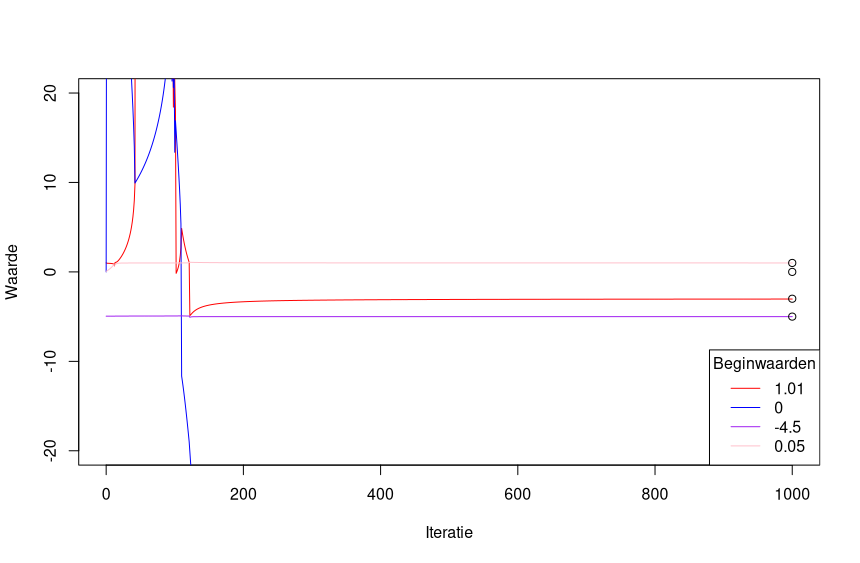
\includegraphics[width=0.9\textwidth]{figures/dkern0}
 \end{subfigure}
  \begin{subfigure}{0.49\textwidth}
  \caption{\(2x^3 - 12x^2 + 18x\)}
  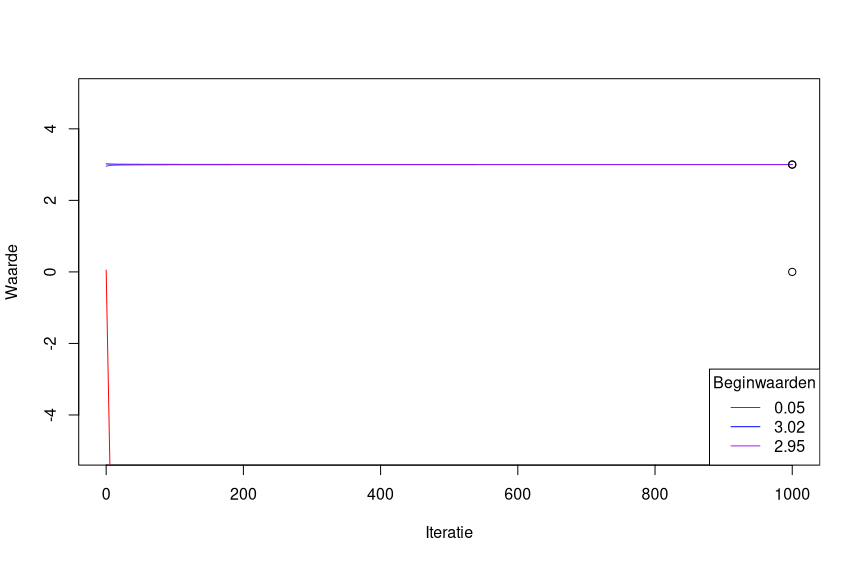
\includegraphics[width=0.9\textwidth]{figures/dkern1}
 \end{subfigure}
\end{figure}

\textbf{Aanpassing noemer:} tot nu toe werd de noemer (\(\prod_{j \neq i}{\left(x^{(n)}_i - x^{(n)}_j\right)}\)) berekend in een for-loop. Dit geeft enkele problemen bij meervoudige nulwaarden: \(x^{(n)}_i\) ligt dan erg dicht bij \(x^{(n)}_j\), dus de noemer wordt erg klein. Indien we de list-comprehension (in combinatie met de \verb|prod| functie)\\
\verb|prod([ 1 if elem == val else (val - elem) for elem in prev ])|\\
gebruiken, worden deze gevallen al gedeeltelijk ge\"elimineerd.

Opvallend is wel dat deze methode minder dicht komt bij de effectieve nulwaarden; ze is meestal slechts tot op 2 of 3 beduidende cijfers correct. Opnieuw helpt de methode waarbij we van ring veranderen, maar dit zorgt ook niet voor de \verb|1e-15| precisie die het andere algoritme haalde.

\subsection{Sage default}
Wanneer we naar de Sage source code kijken (op GitHub); meer specifiek naar het bestand \href{https://github.com/sagemath/sage/blob/de32db6991a5293f037bb35d12890152a8ab99e6/src/sage/rings/polynomial/polynomial_element.pyx}{src/sage/rings/polynomial/polynomial\_element.pyx (lijn 7192)} (de effectieve code start op lijn 7834), dan zien we dat het algoritme bepaald kan worden door de gebruiker (de parameter \verb|algorithm|). Indien dit niet gebeurd, bepaalt Sage zelf het "beste" algoritme. De code is samen te vatten als volgt:
\begin{enumerate}
 \item Indien de ring die de polynoom bevat, zelf een manier heeft om wortels te vinden, gebruik die manier (desnoods met gebruik van \verb|algorithm|).
 \item Indien \verb|algorithm| \verb|'numpy'|, \verb|'either'| of \verb|None| is, gebruik de \verb|numpy| algoritmen (deze geeft een warning wanneer we met getallen met meer dan 53 bits precisie werken). Volgens de \href{https://numpy.org/doc/stable/reference/generated/numpy.roots.html}{numpy documentatie} gebruikt dit de companionmatrix.
 \item Indien het \verb|numpy| algoritme faalt of \verb|algorithm == 'pari'|, gebruik het \verb|pari| algoritme. Volgens de \href{https://pari.math.u-bordeaux.fr/dochtml/html/Polynomials_and_power_series.html#polroots}{pari documentatie} gebruikt dit \href{https://en.wikipedia.org/wiki/Splitting_circle_method}{Sch\"onhage's algoritme}.
\end{enumerate}

\section{Littlewoodveeltermen}
Om de C++ code te testen werd de \href{https://github.com/jay-tux/jtpp}{JT++}-suite gebruikt (zie de bestanden in de \verb|/tests/|-directory).

\subsection{Brute-force}
\subsubsection{Algoritme}
\textbf{CUDA/C++ implementatie:} voor deze implementatie gebruikte ik \href{https://en.wikipedia.org/wiki/Bairstow%27s_method}{Bairstow's Algoritme} ge\"implementeerd in C++ en geaccelereerd door middel van CUDA (op een GeForce GTX1050M). Bairstow's Algoritme berekent de nulwaarden door middel van factorisatie (elke veelterm met re\"ele co\"effici\"enten kan ontbonden worden door factoren van de vorm $(x - a)$ en $(x^2 + bx + c)$ met negatieve discriminant). Hierdoor hoeven alleen berekeningen met re\"ele getallen uitgevoerd te worden. De effectieve code is een variant op \href{https://github.com/PowerUpMasters/BairstowMethod/blob/master/bairstow.py}{dit algoritme}. Hieronder (algoritme 1, volgende bladzijde) staat de gebruikte pseudocode.
\begin{algorithm}
 \KwIn{co\"efficienten (a), graad v/d veelterm (g), beginwaarden (r, s)}
 \KwData{tolerantie (tol)}
 \KwOut{array met nulwaarden}
 $result \gets []$\;
 \If{\(g < 1\)}{
 	\KwRet{result}\;
 }
 \If{\(g == 1\) \KwAnd $a_1 \neq 0$}{
 	$result.add(\frac{-a_0}{a_1})$\;
 	\KwRet{result}\;
 }
 \If{\(g == 2\)}{
 	$a' \gets a_2, b \gets a_1, c \gets a_0$\;
 	$D \gets b^2 - 4a'c$\;
 	$result.add(\frac{\sqrt{D} - b}{2a})$\;
 	$result.add(\frac{-\sqrt{D} - b}{2a})$\;
 	\KwRet{result}\;
 }

 $n \gets deg + 1$\;
 $b \gets [0...0, a_{n-2} + r * a_{n-1}, a_{n-1}]$; \tcp{$deg$ elementen}
 $c \gets [0...0, b_{n-2} + r * b_{n-1}, b_{n-1}]$; \tcp{$deg$ elementen}

 \For{$i \gets n - 3$; $i >= 0$; $i--$}{
 	$b_i = a_i + r*b_{i+1} + s*b_{i+2}$\;
 	$c_i = b_i + r*c_{i+1} + s*c_{i+2}$\;
 }

 $din \gets (c_2^2 - c_3*c_1)^{-1}$\;
 $r \gets r + din * (-c_2*b_1 + c_3*b_0)$\;
 $s \gets s + din * (c_1*b_1 - c_2*b_0)$

 \If{$abs(b_0) > tol$ \KwOr $abs(b_1) > tol$}{
 	$result.add(bairstow(a, g, r, s))$\;
 	\KwRet{result}\;
 }
 \If{$g \geq 3$}{
 	$dis \gets r^2+4s$\;
 	$results.add(\frac{r - \sqrt{dis}}{2})$\;
 	$results.add(\frac{r + \sqrt{dis}}{2})$\;
 	$results.add(bairstow(b[2, ...], r, s, g-2))$\;
 	\KwRet{result}\;
 }
 \KwRet{result}\;
 \caption{Bairstow's algoritme}
\end{algorithm}

Voor de initi\"ele schatting van de kwadratische co\"effici\"enten raadt \href{https://en.wikipedia.org/wiki/Bairstow%27s_method#Example}{Wikipedia} aan om $r = \frac{a_{n-1}}{a_n}; s = \frac{a_{n-2}}{a_n}$ te gebruiken. Bij de Littlewoodveeltermen zullen deze waarden altijd -1 of 1 zijn. Als compromis gebruiken we $r = -1; s = 1$.

\textbf{Optimalisaties tijdens het ontwerp:} een aantal optimalisaties in de code konden al doorgevoerd worden tijdens het ontwerpen van de code zelf:\
\begin{itemize}
 \item De helft van de veeltermen hoeven niet opgelost te worden: $\forall p \in I\!R[x]: \forall x \in I\!R: p(x) = 0 \iff -p(x) = 0$. Dit heeft als voordeel dat een groot deel van de berekeningen niet opgelost hoeft te worden.
 \item Het genereren van de veelterm-arrays kan op de GPU gebeuren (parrallelisme). Hierdoor worden alle veeltermen gelijktijdig gegenereerd van hun index (op basis van de bits in hun index: een 0-bit stelt een co\"effici\"ent -1 voor, terwijl een 1-bit de co\"effici\"ent 1 voorstelt).
\end{itemize}

\subsubsection{Praktische zaken}
\textbf{Moeilijkheden tijdens het schrijven:} de originele berekening van $r$ en $s$ gebruikt een recursieve aanpak. Dit resulteerde echter in een \verb|Segmentation Fault| (veroorzaakt door een stack-overflow). Ik kon dit oplossen door de recursieve call in het \verb|if| blok op lijnen 26-29 te vervangen door een \verb|while| loop. Een andere moeilijkheid werdt gevormd door de oneindige loop die ontstond; deze werd opgelost door na een bepaald aantal pogingen (in te stellen via de \verb|MAX_TRIES| macro) de schatting voor de co\"effici\"enten willekeurig te stellen. Het implementeren van die willekeurige schattingen (op de GPU) bracht ook zijn eigen problemen mee, maar die werden relatief snel opgelost (dankzij \href{https://gist.github.com/NicholasShatokhin/3769635}{Nicholas Shatokhin}). Nadat alle individuele testen slaagden (1 veelterm), zat er nog een grove fout in de implementate: de schattingen van de co\"effici\"enten werden gedeeld tussen de threads. De oplossing hiervoor bestond ervan de schattingen de alloceren en initializeren in de initializatiefase van het algoritme. Dit zorgde voor de volgende initializatie:

\begin{algorithm}[H]
 \KwIn{alle co\"efficienten (a), graad v/d veelterm (g)}
 $modcoeff \gets a[offset]$; \tcp{offset op basis van GPU thread ID}
 \lIf{$g \geq 1$}{$r \gets \frac{modcoeff_{g-1}}{modcoeff_g}$}
 \lElse{$r \gets 1$}
 \lIf{$g \geq 2$}{$s \gets \frac{modcoeff_{g-2}}{modcoeff_g}$}
 \lElse{$s \gets 1$}
 \caption{Initalizatie Bairstow's algoritme}
\end{algorithm}
Verder worden er nog een aantal parameters aangepast zodat alles GPU-gebaseerd kan gebeuren (en dus vele veeltermen tegelijk opgelost kunnen worden).

\textbf{Andere startwaarden:} wanneer het algoritme vastloopt (doordat de startwaarden niet convergeren), werden initieel gewoon nieuwe startwaarden gegenereerd. Dit gaf geen enkele garantie op convergentie. Een manier om dit probleem te proberen beperken was de willekeurige waarden te beperken binnen een bepaald interval. Dit werkte net iets beter, maar verhielp nog niet alles. Na het lezen van \href{https://stackoverflow.com/questions/32201058/bairstows-method-initial-quadratic-approximations}{deze StackOverflow post}, besliste ik om volgende waarden te gebruiken als nieuwe startwaarden:
\begin{align*}
rad &= \sum_{i=0}^{n}{|a_i|} \\
r &= 2 * \pi * rad^2 * cos(rng()) \\
s &= 2 * \pi * rad^2 * sin(rng()) \\
\end{align*}
Dit genereert de veelterm $x^2 + 2*rad^2*\pi*cos(\alpha)x + 2*rad^2*\pi*sin(\alpha)$. Het punt $(r, s)$ ligt op de cirkel met straal $rad = \sum_{i=0}^{n}{|a_i|}$. Deze afstand, de "outer root radius", zorgt ervoor dat de waarden snel convergeren. Een vlugge test gaf een erg verrassend resultaat: voor een veelterm van graad $n$, werden exact $n$ nieuwe paren startwaarden gegenereerd.

\textbf{Testing:} de bairstow code werd erg intensief getest. Een veelvoorkomende zwakte in algoritmen om veeltermen op te lossen zijn meervoudige nulwaarden. Deze toonden zich hier opnieuw een zwakte. De volgende testen zijn hardgecodeerd (in \verb|tests/test_bairstow.cu|; met aangegeven veelterm):
\begin{itemize}
 \item \textbf{Graad 0:} (het programma mag niet crashen)
 \item \textbf{Graad 1:}
 \begin{itemize}
  \item 1 re\"ele wortel: $3x-7 = 0$ (wortel: $\frac{7}{3}$)
 \end{itemize}
 \item \textbf{Graad 2:}
 \begin{itemize}
  \item 2 re\"ele wortels: $3x^2 - 10x - 8 = 0$ (wortels: 4 en $\frac{-2}{3}$)
  \item 2 complexe wortels: $2x^2 + 14x + 25 = 0$ (wortels: $\frac{-7}{2} \pm \frac{1}{2} i$)
 \end{itemize}
 \item \textbf{Graad 3:}
 \begin{itemize}
  \item 2 complexe, 1 re\"ele wortel: $x^3 - x^2 - 41x + 105 = 0$ (wortels: 7 en $\frac{-7}{2} \pm \frac{1}{2} i$)
  \item 3 re\"ele wortels: $x^3 - x^2 - 41x + 105$ (wortels: 3, 5 en -7)
 \end{itemize}
 \item \textbf{Graad 4:}
 \begin{itemize}
  \item 2 paar complexe wortels: $10x^4 - 12x^3 + 8x^2 - 2x + 1/2$ (wortels: $\frac{1}{10} \pm \frac{3}{10} i$ en $\frac{1}{2} \pm \frac{1}{2} i$)
  \item 2 complexe, 2 re\"ele wortels: $2x^4-27x^3+77x^2+263x-795$ (wortels: $7 \pm 2i$, -3 en $\frac{2}{5}$)
  \item 4 re\"ele wortels: $84x^4 + 164x^3 - 608x^2 + 320x$ (wortels: $\frac{5}{7}$, -4, $\frac{4}{3}$ en 0)
 \end{itemize}
\end{itemize}

\textbf{Compilatie:} om het programma te compileren worden volgende tools gebruikt (op 
\includegraphics[height=\fontcharht\font`\B]{figures/arch.png} Arch Linux):
\begin{itemize}
 \item GNU make (om alles gemakkelijk en deel-per-deel te compileren)
 \item G++/GCC (voor de C++/niet-GPU code)
 \item NVCC (voor de GPU/CUDA code)
\end{itemize}

\textbf{Running:} na het volledige littlewood programa te compileren (door middel van \verb|make|), kan het programma gestart worden met of zonder argumenten. De hoeveelheid argumenten is afhankelijk van de buildtime \verb|PROFILING| flag:
\begin{itemize}
 \item Zonder argumenten (\verb|bin/bruteforce|) start het programma en vraagt de gebruiker om de graad van de littlewoodveeltermen. Enkel deze graad wordt gegenereerd en opgelost.
 \item 1 argument (\verb|bin/bruteforce <graad>|; alleen wanneer \verb|PROFILING| niet enabled is) start het programma en lost alle veeltermen van graad $[1, ..., graad[$ op. Indien $graad$ 0 is, zal het programma zoveel mogelijk veeltermen oplossen.
 \item 2 argumenten (\verb|bin/bruteforce <graad> <bestand>|) start het programma analoog aan de optie met 1 argument, maar zal, indien \verb|PROFILING| enabled is, na elke iteratie de profilingdata naar het bestand schrijven.
\end{itemize}

\textbf{Rendering:} het littlewood-programma zelf (dmv de Makefile te compileren naar \verb|bin/bruteforce|) schrijft de oplossingen naar \verb|stdout|. Door deze stream om te leiden naar \verb|res.txt|, verkrijgen we een dataset met platte tekst voor de resultaten (1 oplossing per lijn). Deze kunnen we door middel van een eenvoudig R script plotten:
\begin{lstlisting}[language=R]
data <- read.csv('/path/to/file', header=F, sep=' ')
plot(c(-2,2), c(-2,2), main="Littlewood Polynomial Roots",
	col='white', xlab='Re(x)', ylab='Im(x)')
points(data)
\end{lstlisting}

\subsubsection{Toekomst}
\textbf{Adaptief renderen:} eigenlijk zou een OpenGL programma in staat moeten zijn om deze resultaten dan (via stream of van een bestand) mooi zelf te renderen. Pogingen om dit te doen resulteerden helaas in vooral mislukkingen.

\textbf{Verdere optimalisaties:} de code op zich is nog niet optimaal. Een aantal dingen kunnen nog verbeterd worden:\
\begin{itemize}
 \item Een veelterm van graad $n$ kan voorgesteld worden als een \verb|int a|  met $0 \leq a \leq 2^{n}$ ($n+1$ co\"effici\"enten, maar slechts $n$ ervan hoeven gebruikt te worden, zie hierboven), waarbij de 0-bits gebruikt worden als co\"effici\"ent -1 en de 1-bits gebruikt worden als co\"effici\"ent 1.
\end{itemize}

\subsubsection{Resultaten}
\textbf{Profiling:} de littlewood programma bevat ingebouwde functionaliteit om de duur van de operaties te meten (indien de \verb|PROFILING| preprocessor directive gedefinieerd is at buildtime).

\subsection{Per-pixel}
\subsubsection{Bewijzen}
In de bewijzen en eigenschappen wordt $L[x]$ gebruikt als de verzameling van de Littlewoodveeltermen, met andere woorden: $p(x) \in L[x] \iff (p(x) = \sum_{i=0}^{n}{a_ix^i} \land \forall i \in \{0, 1, ..., n\}: a_i \in \{ -1, 1\})$. Verder wordt de notatie $z \in \mathbb{C}_{<1}$ gebruikt voor $z \in \mathbb{C} \land |z| < 1$.
\begin{enumerate}
\item \underline{$\forall z \in \mathbb{C}_{<1}: \forall l(x) \in L[x]: |l(z)| \leq \frac{1}{1-|z|}$} \newline
\textbf{Bewijs:}
\begin{align*}
|l(z)| &\leq l(|z|) &\text{ (wegens l(x) is een som en } |a+b| \leq |a| + |b| \text{)} \\
&\leq l_{max}(|z|) &\text{ (} |z| \text{ is een positief, re\"eel getal, dus } l_{max} = \sum_{i = 0}^{\infty}{x^i} \text{)} \\
&= \lim_{t \to \infty}{\sum_{i = 0}^{t}{|z|^i}} &\text{ (met } 0 < |z| < 1 \text{)} \\
&= \frac{1}{1-|z|} &\text{ (reekssom van een meetkundige reeks)}
\end{align*}


\item \underline{$\forall z \in \mathbb{C}: (\exists l(x) \in L[x]: l(z) = 0) \implies (\exists l'(x) \in L[x]: l(z^{-1}) = 0)$} \newline
\textbf{Bewijs:} (door constructie van $l'$)
\begin{align*}
l(x) &= \sum_{i = 0}^{n}{a_ix^i} \text{, met } l(z) = 0 \land a_0 \neq 0 &\text{(def. littlewood)} \\
\text{neem } l'(x) &= x^n * l(x^{-1}) = x^n * \sum_{i = 0}^{n}{a_ix^{-i}} = \sum_{i = 0}^{n}{a_ix^{n-i}} \\
&\Downarrow \\
l'(z^{-1}) &= (z^{-n}) * l((z^{-1})^{-1}) = (z^{-n}) * l(z) = (z^{-n}) * 0 \\
&= 0
\end{align*}

\item \underline{$\forall (z, l(x)) \in \mathbb{C}_{<1} \times L[x], d = gr(l(x)): (|l(z)| > \frac{|z|^{d+1}}{1 - |z|})$} \newline \underline{$\implies \neg(\exists l'(x) \in L[x]: l' \text{ is een uitbreiding van } l \land l'(z) = 0)$} \newline
\textbf{Bewijs:} (uit het ongerijmde; stel $\exists l' \in L[x]: l'(z) = 0$)
\begin{align*}
 0 = l'(z) &= l(z) + \sum_{i=d+1}^{n}{c'_iz^i}
 = \sum_{i=0}^{d}{c_iz^i} + \sum_{i=d+1}^{n}{c'_iz^i} \\
 &\Big\Updownarrow \\
 \sum_{i=0}^{d}{c_iz^i} &= -\sum_{i=d+1}^{n}{c'_iz^i} \\
 &\Big\Downarrow \\
 \frac{\left|z\right|^{d+1}}{1-\left|z\right|} &\sgntxt{<}{(1)} \left|\sum_{i=0}^{d}{c_iz^i}\right| = \left|\sum_{i=d+1}^{n}{c'_iz^i}\right| \\
 &\Big\Updownarrow \\
 \frac{\left|z\right|^{d+1}}{1-\left|z\right|} &< \left|\sum_{i=d+1}^{n}{c'_iz^i}\right|
 \sgntxt{\leq}{(2)} \sum_{i=d+1}^{n}{\left|c'_iz^i\right|}
 \sgntxt{=}{(3)} \sum_{i=d+1}^{n}{\left|z^i\right|}
 \sgntxt{=}{(4)} \sum_{i=d+1}^{n}{\left|z\right|^i} \\
 \frac{\left|z\right|^{d+1}}{1-\left|z\right|} &< \sum_{i=d+1}^{n}{\left|z\right|^i} \\
 &\Big\Updownarrow \\
 \left|z\right|^{d+1} &\leq (1-\left|z\right|) * \sum_{i=d+1}^{n}{\left|z\right|^i}
 = \sum_{i=d+1}^{n}{\left|z\right|^i} - \sum_{i=d+1}^{n}{\left|z\right|^{i+1}} \\
 &= \left|z\right|^{d+1} + (\left|z\right|^{d+2} - \left|z\right|^{d+2}) + \mathellipsis + (\left|z\right|^{n} - \left|z\right|^{n}) - \left|z\right|^{n+1} \\
 &= \left|z\right|^{d+1} - \left|z\right|^{n+1} \\
 &\Big\Updownarrow (5) \\
 z &= 0 \text{ }\sim\text{ Tegenstrijdigheid: } z=0 \text{ is nooit een oplossing voor een } l_n(x) \in L[x]
\end{align*}
\textbf{Gebruikte hulpstellingen:}
\begin{align*}
& \text{1)} & l(x) &> \frac{\left|z\right|^{d+1}}{1 - \left|z\right|} &\text{(gegeven)}\\
& \text{2)} & \forall c \in \mathbb{C} &: \left|a+b\right| \leq \left|a\right| + \left|b\right|\\
& \text{3)} & c_i \in \{-1, 1\} &\implies (c_iz^i) \in \{-z^i, z^i\} \implies \left|c_iz^i\right| = \left|z^i\right| \\
& \text{4)} & \left|z^i\right| &= \left|\prod_{j=1}^{n}{z}\right| = \prod_{j=1}^{n}{\left|z\right|} = \left|z\right|^i \\
& \text{5)} & \left|z\right|^a \geq 0 &\implies (\left|z\right|^{d+1} = \left|z\right|^{d+1} - \left|z\right|^{n+1} \iff z = 0)
\end{align*}
\end{enumerate}

\subsubsection{Algoritme}
Behalve de gegeven stellingen, werd ook gebruik gemaakt van stellingen uit \href{https://fse.studenttheses.ub.rug.nl/12857/1/Scriptie__new_.pdf}{Majken Roelfszema's thesis}, meer bepaald: (haar thesis maakt gebruik van volgende notatie: $D = \{ z | z \in \mathbb{C} \land \exists l(x) \in L[x]: l(z) = 0 \}$)
\begin{enumerate}
 \item \textbf{Stelling 1:} $\forall z \in D: \frac{1}{2} < \left|z\right| < 2$ (met $D$ de verzameling van alle nulwaarden van alle littlewoodveeltermen.
 \item \textbf{Stelling 2:} $D$ is symmetrisch in de re\"ele as, de imaginaire as en de eenheids\-cirkel.
 \item \textbf{Stelling 20:} $\{ z \in \mathbb{C}, \left|z\right| \in [ \frac{1}{\sqrt[4]{2}}, \sqrt[4]{2} ] \} \subset \overline{D}$, waarbij $\overline{D}$ ook de oplossingen van $\lim_{deg(l) \to \infty}{l(x)}$ ($l(x)$ is een littlewoodveelterm) bevat.
\end{enumerate}

Met behulp van deze stellingen kan een relatief eenvoudig algoritme uitgewerkt worden waarbij eerst een paar "basisgevallen" overlopen worden, waarna een eenvoudige \verb|while|-loop zal proberen om een veelterm op te stellen die zichzelf corrigeert richting 0: voor elke volgende graad kunnen slechts 2 co\"effici\"enten toegevoegd worden aan de veelterm: 1 of -1. De co\"effici\"ent die de ervoor zorgt dat de modulus van het resultaat het kleinst wordt, zal opnieuw gebruikt worden in de volgende iteratie. De lus stopt op het moment dat een oplossing is gevonden, de voorwaarde uit het laatste bewijs waar wordt voor beide co\"effici\"enten, of de volgende term kleiner wordt in modulus dan de tolerantie. Met andere woorden, het algoritme probeert (beginnend van de veelterm $l(x) = 1 \in L[x]$) telkens zoveel mogelijk te corrigeren richting 0. Dit is mogelijk als en slechts als geldt dat $0 \leq \left|z\right| < 1$. Om dit te doen kloppen, controleren we of in $\frac{1}{z}$ een veelterm gegenereerd kan worden. Door middel van de stellingen 1 en 20 uit de gelinkte thesis, kunnen we relatief eenvoudig voor een groot aantal punten al bepalen of ze al dan niet kunnen bestaan.

\textbf{Een initi\"ele optimalizatie: } de waarde $\left|a+bi\right|$ wordt in het algoritme meermaals berekend. Aangezien $\left|a+bi\right| = \sqrt{a^2 + b^2}$ een vierkantswortel bevat (en dit een dure operatie is), zullen we in de praktijk de wortel zoveel mogelijk proberen wegwerken. Bij de meeste vergelijkingen kunnen we gewoon beide leden kwadrateren, omdat met constanten gewerkt wordt. Voor de vergelijkingen in lijn 23 ($\left|low\right| > norm \land \left|high\right| > norm$; met $low = c+di, high = e+fi, norm = \frac{\left|a+bi\right|^{d+1}}{1 - \left|a+bi\right|}$) is dit net iets minder eenvoudig (een analoge afleiding kan gebruikt worden voor $high > norm$):
\begin{align*}
 low > norm &\iff \left|c+di\right| > norm \\
 &\iff \sqrt{c^2 + d^2} > \frac{\sqrt{a^2 + b^2}^{d+1}}{1 - \sqrt{a^2 + b^2}} & \\
 &\iff c^2 + d^2 > \frac{\sqrt{a^2 + b^2}^{2(d+1)}}{\left(1 - \sqrt{a^2 + b^2}\right)^2} = \frac{\left(a^2 + b^2\right)^{d+1}}{1 - 2\sqrt{a^2 + b^2} + a^2 + b^2}
\end{align*}
Een laatste plaats waar de wortel niet weggewerkt kan worden is in de uitdrukking $\frac{1}{z} = \frac{1}{a+bi} = \frac{a}{\left|a+bi\right|} + \frac{-b}{\left|a+bi\right|}i = \frac{a}{\sqrt{a^2 + b^2}} + \frac{-b}{\sqrt{a^2 + b^2}}i$.

\begin{algorithm}
 \KwIn{Coordinate of the OpenGL fragment ($(x,y)$)}
 \KwData{tolerance for the algorithm ($tol$)}
 \KwOut{True if $\exists l(x) \in L[x]: l(x + yi) = 0$, otherwise False}
 $a \gets x$, $b \gets y$\;
 \If{$\left|a + bi\right| \leq \frac{1}{2} \lor \left|a + bi\right| \geq 2$}{
  \KwRet{False}; \tcp{Theorem 1 from the linked thesis}
 }
 \If{$a < 0$}{
  \KwRet{isSolution(-a, b)}; \tcp{Theorem 2 from the linked thesis}
 }
 \If{$b < 0$}{
  \KwRet{isSolution(a, -b)}; \tcp{Theorem 2 from the linked thesis}
 }
 \If{$\left|a+bi\right| > 1$}{
  \KwRet{isSolution($\frac{a}{\left|a+bi\right|}$, $\frac{-b}{\left|a+bi\right|}$)}; \tcp{Theorem 2.2.1.2}
 }
 $curr \gets a + bi, px \gets 1, norm \gets \frac{\left|a + bi\right|}{1 - \left|a + bi\right|}$\;
 \While{$\left|curr\right| > tol$}{
  $low \gets px - curr, high \gets px + curr$\;
  \If{$\left|low\right| \leq tol \lor \left|high\right| \leq tol$}{
   \KwRet{True}; \tcp{We found a polynomial}
  }
  \If{$\left|low\right| > norm \land \left|high\right| > norm$}{
   \KwRet{False}; \tcp{Neither way will get a solution}
  }
  $curr \gets curr * (a + bi), norm \gets norm * \left|a + bi\right|$\;
  \If{$\left|low\right| < \left|high\right|$}{
   $px \gets low$
  }
  \Else{
   $px \gets high$
  }
 }
 \KwRet{False}; \tcp{The result doesn't change anymore}
 \caption{$isSolution(x, y)$}
\end{algorithm}

\textbf{Uitzondering:} indien $\left|z\right| = 1$ zal dit algoritme over het algemeen niet convergeren. Door middel van stelling 7 uit M. Roelfszema's thesis ($\forall r \in \mathbb{Q}: e^{i\pi r} \in D$) kunnen we stellen dat elk punt met $1 - tol \leq \left|z\right| \leq 1 + tol$ op de eenheidscirkel ligt en er een $r \in \mathbb{Q}$ bestaat waarvoor $z = e^{i\pi r}$; wat dus betekent dat elk punt op de eenheidscirkel kan meetellen als nulwaarde.

\subsubsection{Hardware limitatie}
Huidige (NVIDIA) GPUs ondersteunen geen \verb|branch prediction|, met andere woorden, elke conditionele jump is een enorm dure operatie op een GPU. Dit zorgt ervoor dat de \verb|while|-loop uit de pseudocode enorm ineffici\"ent en traag is. Indien het aantal iteraties tijdens het compileren al gekend is, kan de compiler een techniek toepassen die \verb|loop unrolling| heet. Deze techniek bestaat eruit elke jump te elimineren door elke iteratie lineair na elkaar in de bytecode te zetten. Het aantal iteraties dat een $z \in \mathbb{C}, \left|z\right| < 1$ nodig heeft om gelijk aan $tol$ te worden, kan eenvoudig berekend worden:

\begin{align*}
\left|z^n\right| = tol \iff \left|z\right|^n = tol \iff n = \log_{\left|z\right|}{tol}
\end{align*}

Met andere woorden, het aantal iteraties is afhankelijk van de tolerantie (het is ook diezelfde tolerantie die bepaald of $z$ veel verandert of niet). Om een gangbare waarde te vinden werd het algoritme ook eens op de CPU uitgevoerd, waarbij het aantal iteraties gelogd werd (elke keer werden 1024x1024 punten berekend).
\begin{figure}[!htb]
 \caption{Aantal iteraties (CPU) $z \in \{ a + bi | a, b \in [ -2, 2 ] \}$}
 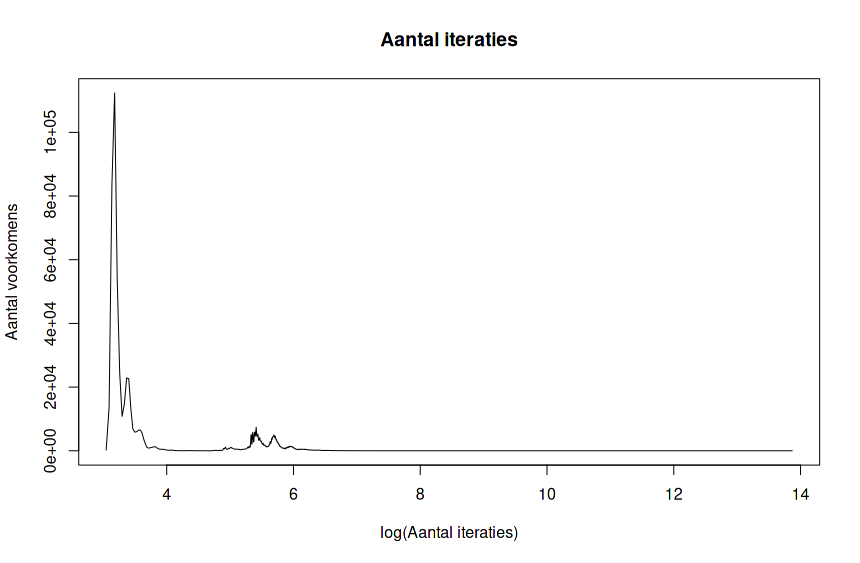
\includegraphics[width=0.45\textwidth]{figures/gl-iteraties}
 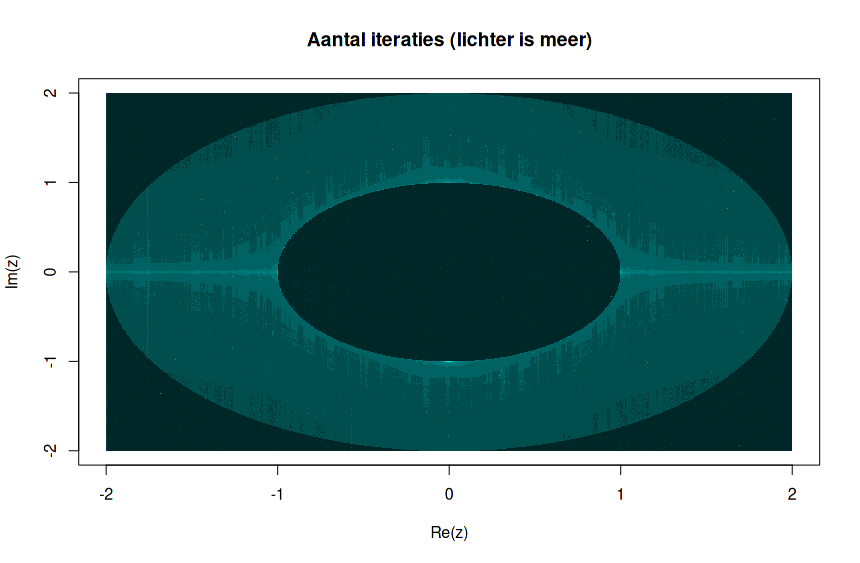
\includegraphics[width=0.45\textwidth]{figures/glit-complex}
 \caption{Aantal iteraties (CPU, ingezoomd)}
 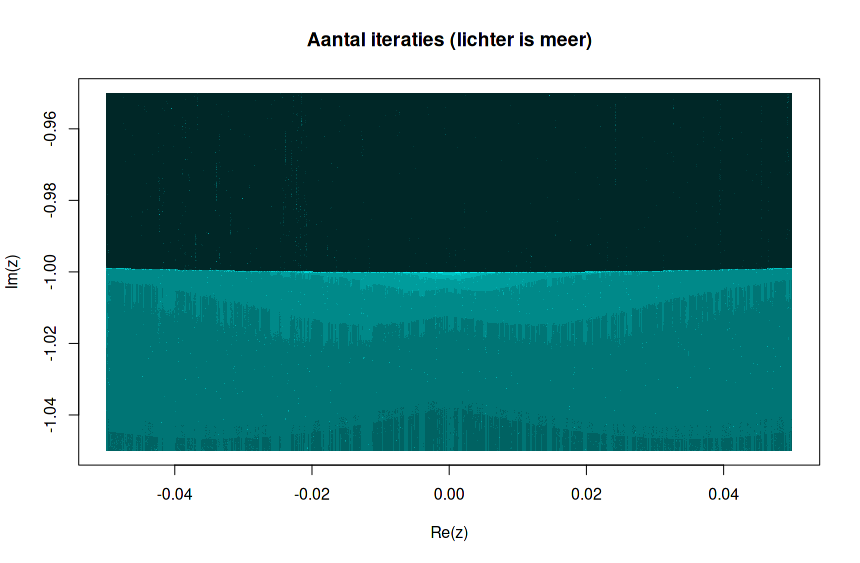
\includegraphics[width=0.45\textwidth]{figures/zoomed_itcomplex}
 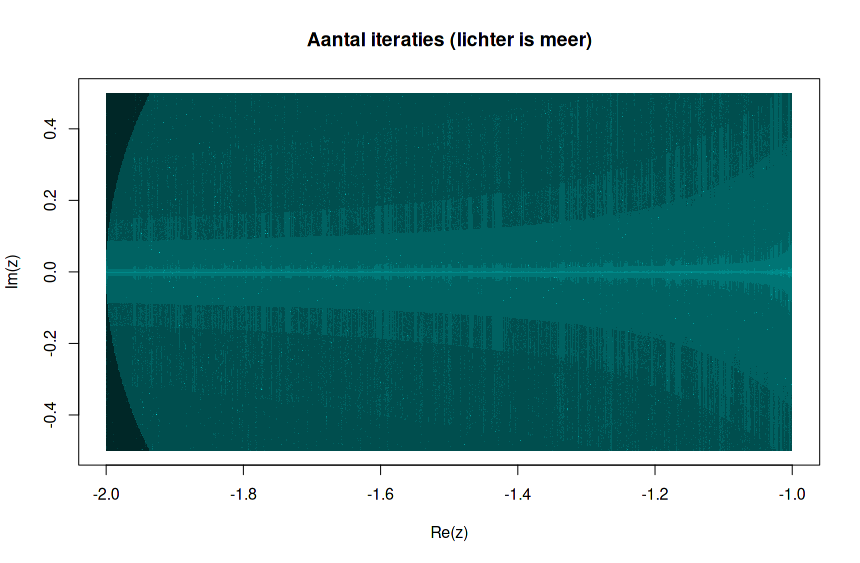
\includegraphics[width=0.45\textwidth]{figures/semizoomed}
\end{figure}
Uit deze plots blijkt dat de complexe getallen die het meeste iteraties nodig hebben, zich bevinden op de assen, dicht bij $\left|z\right| \sim 1$. Om tot een goede schatting te komen, werd eens ingezoomd op de gebieden $z \in \{a + bi | a \in [ -0.05, 0.05 ], b \in [ -1.05, -0.95 ]\}$ en $z \in \{ a + bi | a \in [ -2, -1 ], b \in [ -0.5, 0.5 ]\}$.

Aangezien dit aantal erg groot kan worden, zal deze shader heel snel heel ineffici\"ent en traag worden. We kunnen hierrond door CUDA en OpenGL samen te laten werken, waarbij de CUDA kernel zijn resultaten zal "renderen" naar een texture, en OpenGL deze texture zal gebruiken bij het renderen van een fragment. Deze texture zal 4096 horizontale en 4096 verticale samples bevatten zodat de OpenGL context nooit zal moeten extrapoleren tijdens het renderen. Hierdoor ziet de uiteindelijke render loop er ruwweg als volgt uit: \\

\begin{algorithm}[H]
 \text{Set up OpenGL}\;
 \text{Link OpenGL texture to CUDA}\;
 \While{\text{Not yet exiting}}{
  \text{Handle input}\;
  \If{Input changed position/scale}{
   \text{Use CUDA kernel to generate texture}\;
   \text{Synchronize GPU}\;
  }
  \text{Set up frame (OpenGL calls)}\;
  \text{Swap OpenGL buffers}\;
  \caption{Render loop/driver code}
 }
\end{algorithm}

Om deze complexe samenwerking tot een goed einde te brengen, werd gebruik gemaakt van \href{https://github.com/Forceflow/cuda2GLcore}{Forceflow/cuda2GLcore}. De uiteindelijke implementatie kan arbitrair snel (of arbitrair exact) werken, enkel gelimiteerd door hardware en de IEEE \verb|float| specificatie.

\subsubsection{Uiteindelijke applicatie}
\textbf{Compilatie:} net zoals bij vorig deel is ook hier een Makefile meegeleverd zodat de code snel en eenvoudig gebouwd kan worden. De code heeft dependencies op:
\begin{enumerate}
 \item GNU Make (om deel per deel te compileren)
 \item NVCC (de NVIDIA compiler), en G++ (om niet-CUDA code te compileren)
 \item CUDA en de CUDA SDK (\verb|cuComplex|) voor de eigenlijke berekeningen
 \item OpenGL ($\geq 4.6$ Core), GLEW, GLFW (voor het renderen). Hierbij horen ook de X11 libraries (X11, Xrandr, Xi).
\end{enumerate}

\textbf{Controls:} wanneer de applicatie niet aan het rekenen is, kunnen de volgende toetsen gebruikt worden om de camera te besturen. Indien de camera aangepast is, zal het frame erna de resulterende afbeelding opnieuw berekend worden.
\begin{enumerate}
 \item \textit{W, S:} beweeg de camera naar boven, resp. onder
 \item \textit{A, D:} beweeg de camera naar links, resp. rechts
 \item \textit{Q, E:} zoom uit, resp. in
 \item \textit{Spatie:} reset de camera
 \item \textit{Escape:} sluit de applicatie
\end{enumerate}
Het beeld toont elke frame op de linkerzijde (in het rood) de verzameling $D$ (de oplossingen) en op de rechterzijde (in het blauw) het aantal iteraties dat nodig was om tot die oplossing te komen.
Om de complexe getallen te berekenen die overeenkomen met de pixels wordt volgende formule gebruikt ($zoom$ en $center$ zijn eigenschappen van de camera, waarbij $zoom$ groter wordt naarmate verder ingezoomd wordt en waar $center$ het complex getal op de middelste pixel voorstelt).
\begin{align*}
 \mathcal{T}: &[0, w]\times[0, h] \to CamSpace:& \\
 &(x, y) \to (\frac{4 * x}{w * zoom} - \frac{2}{zoom} + Re(center), \frac{4 *y}{h * zoom} - \frac{2}{zoom} + Im(center))
\end{align*}

\textbf{Snelheid:} zoals eerder vermeld is de snelheid van de implementatie afhankelijk van twee factoren: het maximaal aantal iteraties en de precisie. Onder "basisomstandigheden" ($2^{20}$ iteraties, precisie $1 * 10^{-20}$, standaardcamera), haalt de applicatie ongeveer een 0.2 fps (dus ongeveer 5s om de volledige afbeelding te renderen), indien de kernel berekend moet worden. Onder idle (geen aanpassingen in de camera), haalt de applicatie een 60-tal FPS (dit is het harde limiet dat door GLFW wordt opgelegd). De implementatie werd ook geprofileerd bij andere instellingen. Het profileren kan opnieuw aangepast worden door middel van macros (\verb|PROFILING| om de profilering aan of uit te zetten. Indien \verb|#if PROFILING| worden de precisies in [\verb|MIN_PRC|, \verb|MAX_PRC|] getest door telkens de precisie met \verb|DELTA_PRC| te vermenigvuldigen; het aantal iteraties kan analoog aangepast worden door middel van \verb|MIN_IT|, \verb|MAX_IT| en \verb|DELTA_IT|; elke combinatie van precisie en iteraties word \verb|REPEATS| keer getest).

In figuren 5 en 6 wordt deze data geplot, waarbij elke kleur zijn eigen betekenis heeft; groen stellen de minima voor, grijs de gemiddelden, blauw de medianen en rood de maxima. Alle grafieken gebruiken een logaritmische schaal (met basis 10 voor de precisie en basis 2 voor het aantal iteraties) om de data mooi over de x-as te verdelen. Deze basissen zijn zo gekozen omdat dit ook gereflecteerd wordt in de waarden (het aantal iteraties evolueerde tijdens het genereren van de data door middel van bitshifts (\verb|1 << x|), terwijl voor de precisie telkens de exponent in de wetenschappelijke notatie aangepast werd (\verb|1e-x|)).

Telkens wordt \'e\'en van beide parameters genomen om te vergelijken met een paar waarden van de andere, om zo te kunnen uitzetten tegenover de fps.

Wanneer de precisie uitgezet wordt, blijkt dat deze ofwel erg grillig is, ofwel relatief constant. Enkel wanneer het aantal iteraties erg groot wordt, krijgen we een meer "verwachtte" grafiek: de fps groeit naarmate het de precisie daalt (naarmate de threshold groter wordt).

Het aantal iteraties toont een heel ander beeld: de grafiek is telkens erg gelijkaardig, met waarden die (zo goed als) altijd erg dicht bij elkaar liggen (de meeste lijnen overlappen).

Figuur 7 zet alle gegevens tegenover elkaar uit: op de x-as vinden we telkens de precisie terug (in $\log_{10}$ om een gelijkmatige spreiding te bekomen), op de y-as het maximaal aantal iteraties (opnieuw in $\log_2$) en de behaalde fps wordt (als $\log_2$) gekleurd waarbij rood laag is, blauw gemiddeld en groen hoog (relatief gezien). Deze figuren tonen aan dat de bepalende factor niet zozeer de precisie als wel het maximaal aantal iteraties is.

\begin{figure}[!htb]
 \caption{FPS/Precisie-plots ($\log_{10}(prec)$)}
 \begin{subfigure}{0.49\textwidth}
  \caption{Overzicht van alle statistieken}
  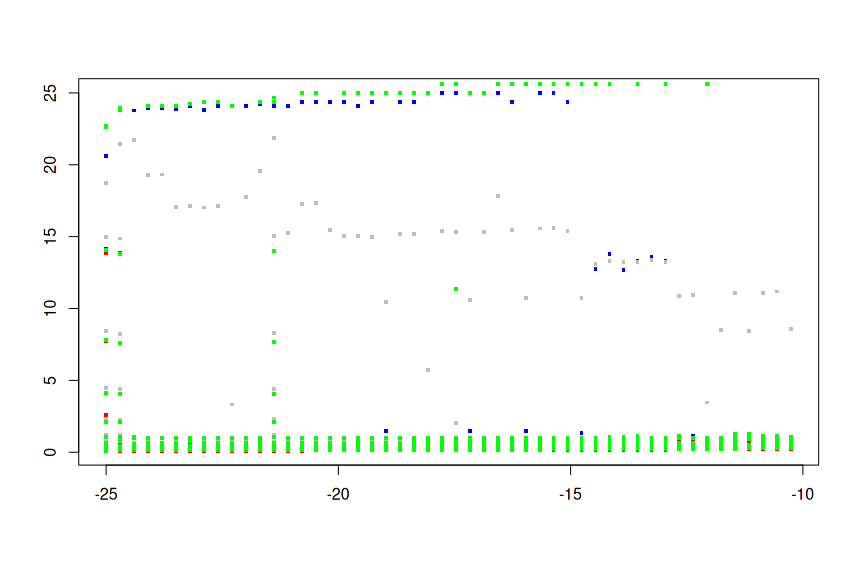
\includegraphics[width=0.95\textwidth]{elegant-gl/datasets/plot_prec}
 \end{subfigure}
 \begin{subfigure}{0.49\textwidth}
  \caption{Bij 1024 ($1 << 10$) iteraties}
  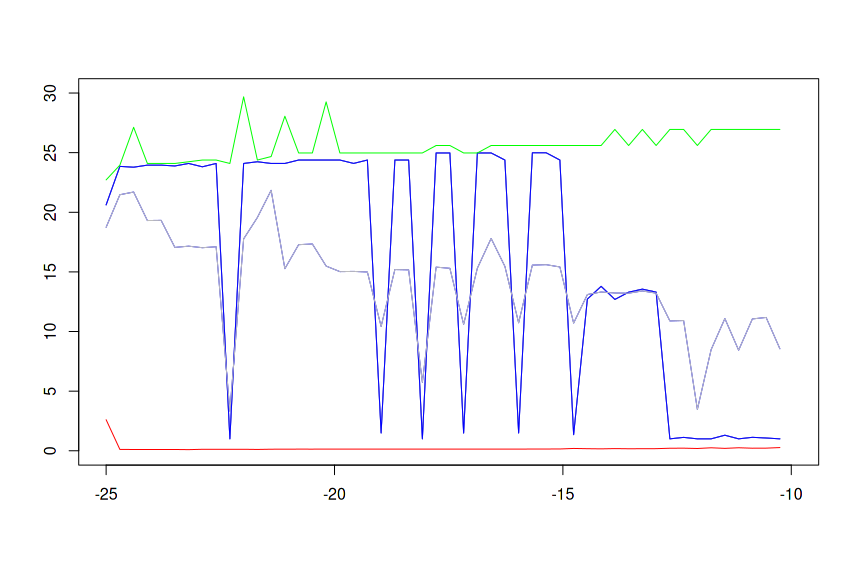
\includegraphics[width=0.95\textwidth]{elegant-gl/datasets/plot_prec_1024it}
 \end{subfigure}
 \begin{subfigure}{0.49\textwidth}
  \caption{Bij 16384 ($1 << 14$) iteraties}
  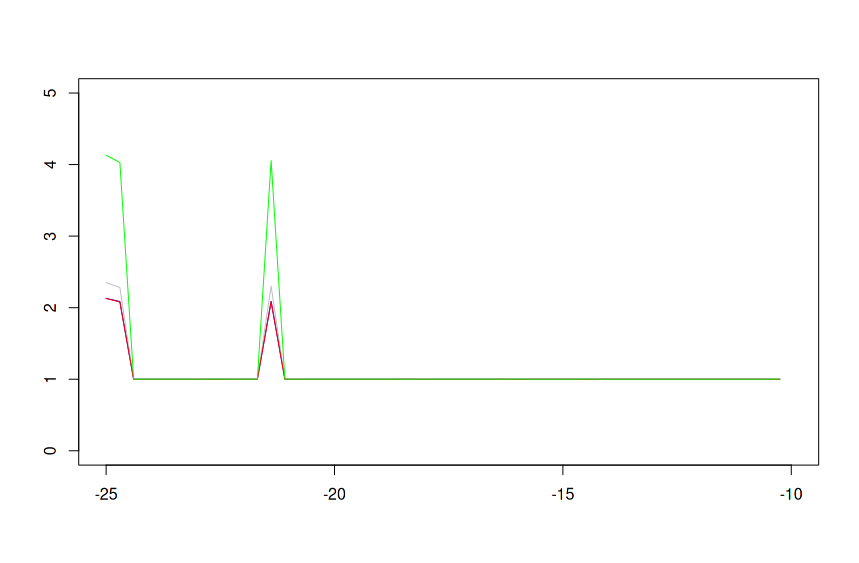
\includegraphics[width=0.95\textwidth]{elegant-gl/datasets/plot_prec_16384it}
 \end{subfigure}
 \begin{subfigure}{0.49\textwidth}
  \caption{Bij 33554432 ($1 << 25$) iteraties}
  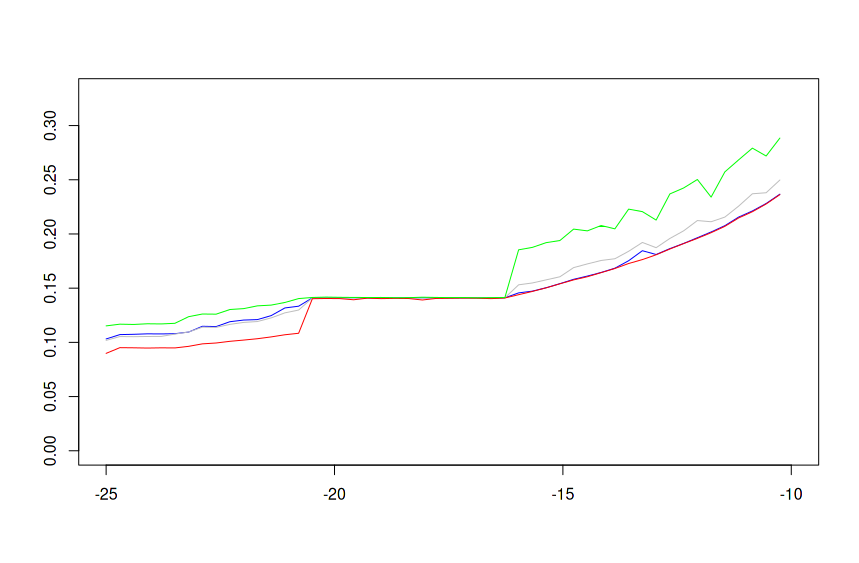
\includegraphics[width=0.95\textwidth]{elegant-gl/datasets/plot_prec_33554432it}
 \end{subfigure}
\end{figure}

\begin{figure}[!htb]
 \caption{FPS/maximaal aantal iteraties ($\log_2(it)$)}
 \begin{subfigure}{0.49\textwidth}
  \caption{Overzicht van alle statistieken}
  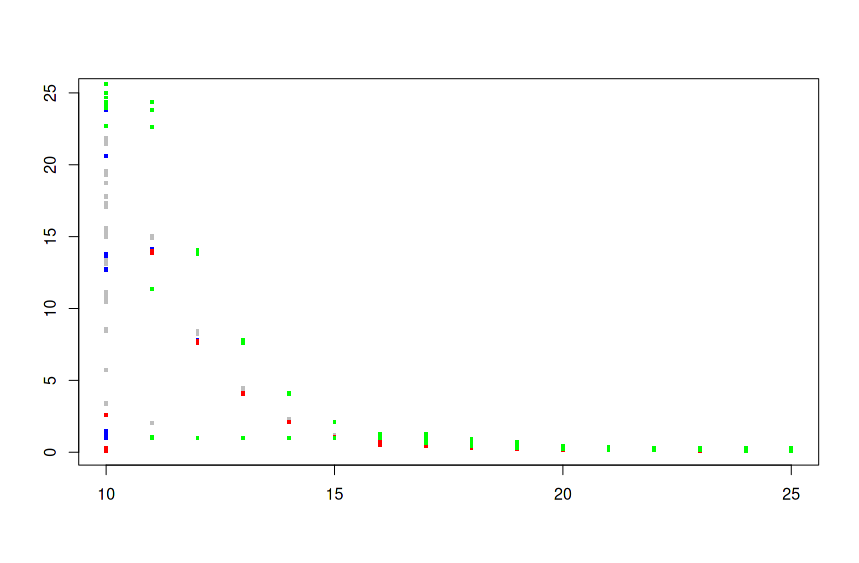
\includegraphics[width=0.95\textwidth]{elegant-gl/datasets/plot_it}
 \end{subfigure}
 \begin{subfigure}{0.49\textwidth}
  \caption{Bij precisie $8*10^{-25}$}
  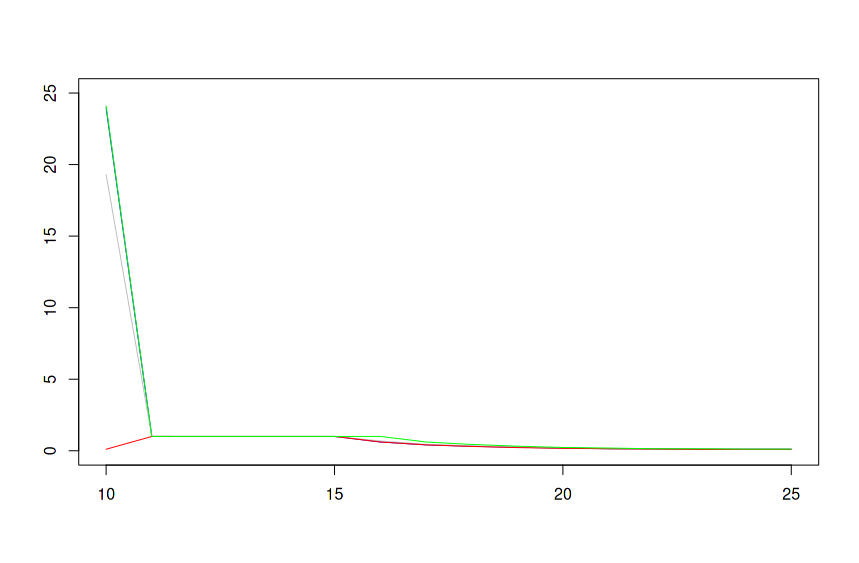
\includegraphics[width=0.95\textwidth]{elegant-gl/datasets/plot_it_8e-25prec}
 \end{subfigure}
 \begin{subfigure}{0.49\textwidth}
  \caption{Bij precisie $5.6295*10^{-11}$}
  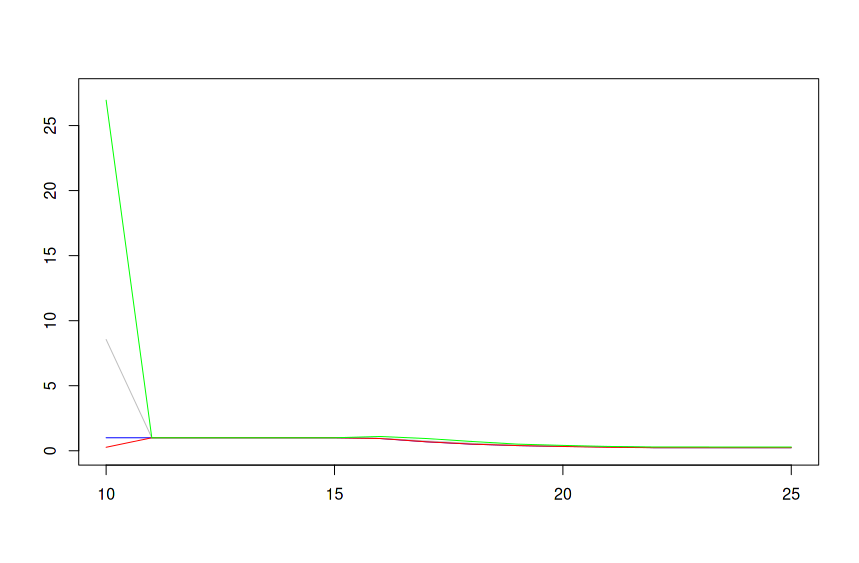
\includegraphics[width=0.95\textwidth]{elegant-gl/datasets/plot_it_5.6295e-11prec}
 \end{subfigure}
 \begin{subfigure}{0.49\textwidth}
  \caption{Bij precisie $2.14748*10^{-16}$}
  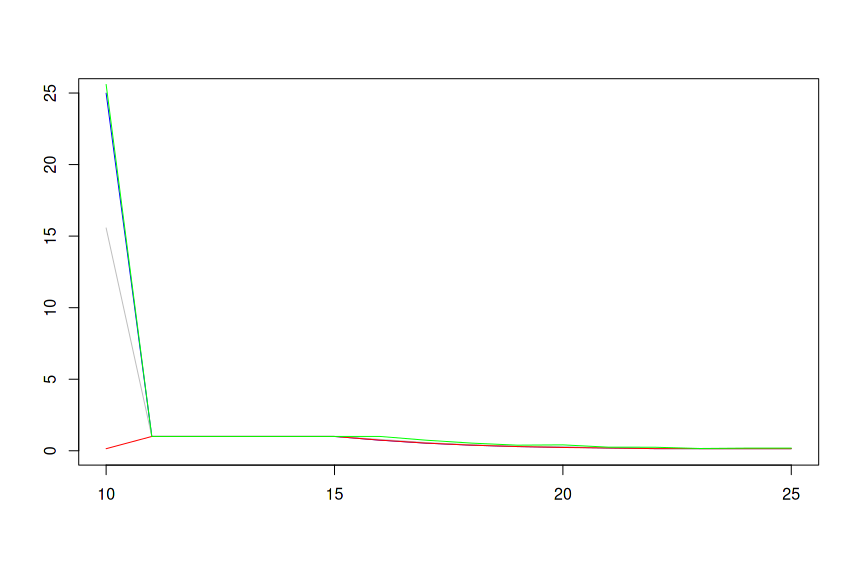
\includegraphics[width=0.95\textwidth]{elegant-gl/datasets/plot_it_2.14748e-16prec}
 \end{subfigure}
\end{figure}

\begin{figure}[!htb]
 \caption{FPS t.o.v. beide parameters; $\log_2(fps)$, $x=\log_{10}(prec)$, $y=\log_{2}(it)$}
 \begin{subfigure}{0.49\textwidth}
  \caption{Minimum}
  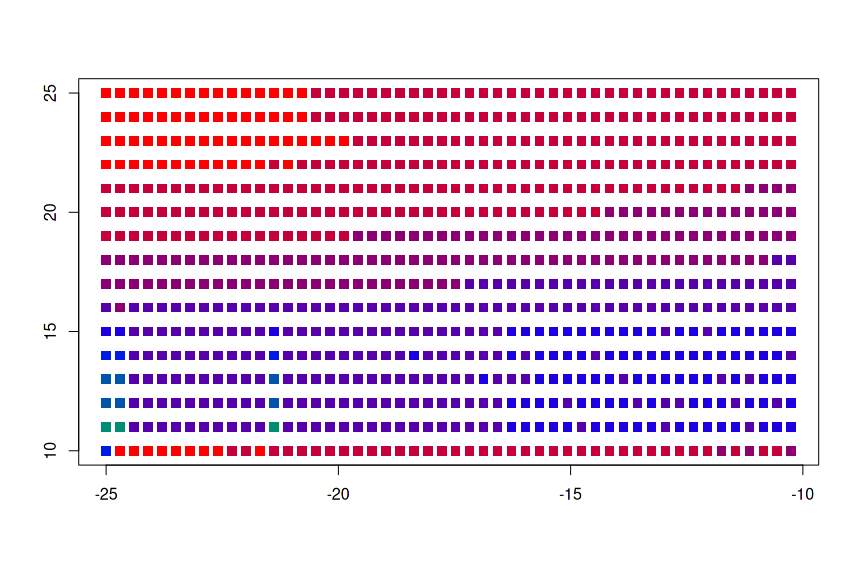
\includegraphics[width=0.95\textwidth]{elegant-gl/datasets/colors_min}
 \end{subfigure}
 \begin{subfigure}{0.49\textwidth}
  \caption{Gemiddelde}
  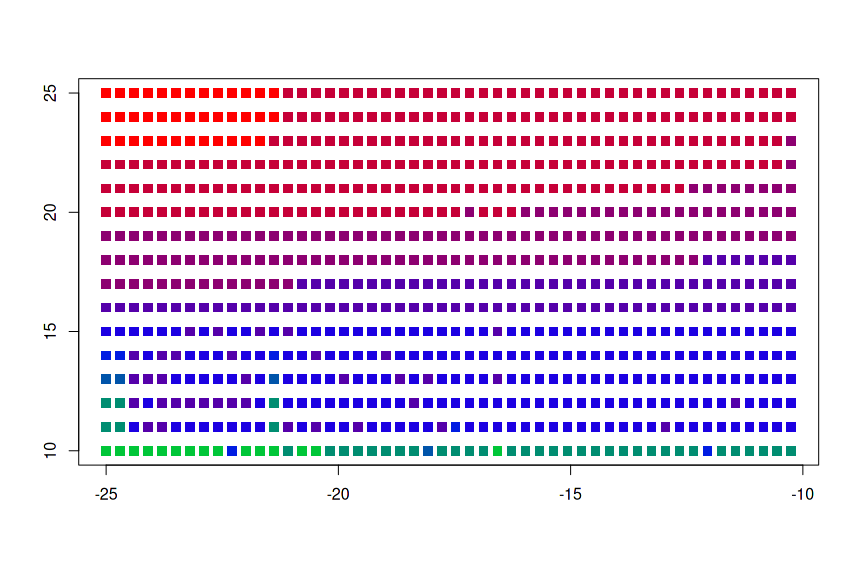
\includegraphics[width=0.95\textwidth]{elegant-gl/datasets/colors_mean}
 \end{subfigure}
 \begin{subfigure}{0.49\textwidth}
  \caption{Mediaan}
  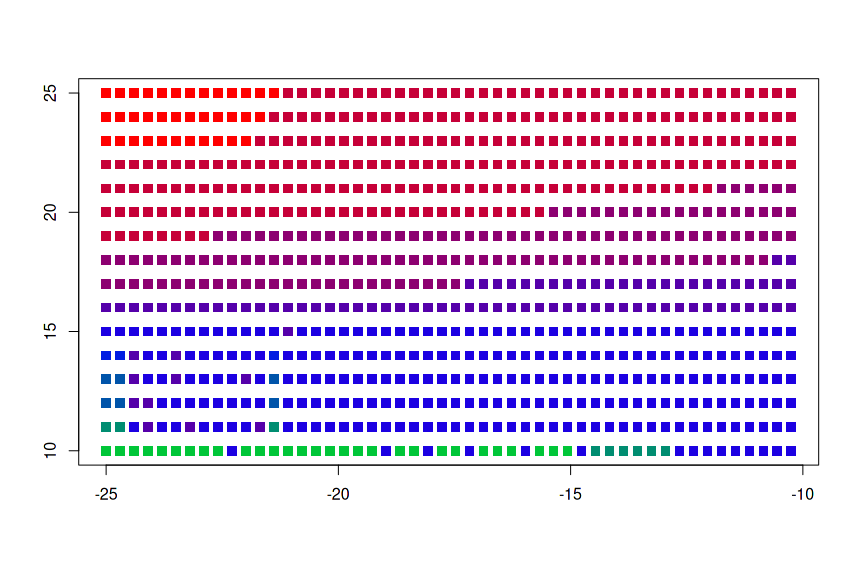
\includegraphics[width=0.95\textwidth]{elegant-gl/datasets/colors_median}
 \end{subfigure}
 \begin{subfigure}{0.49\textwidth}
  \caption{Maximum}
  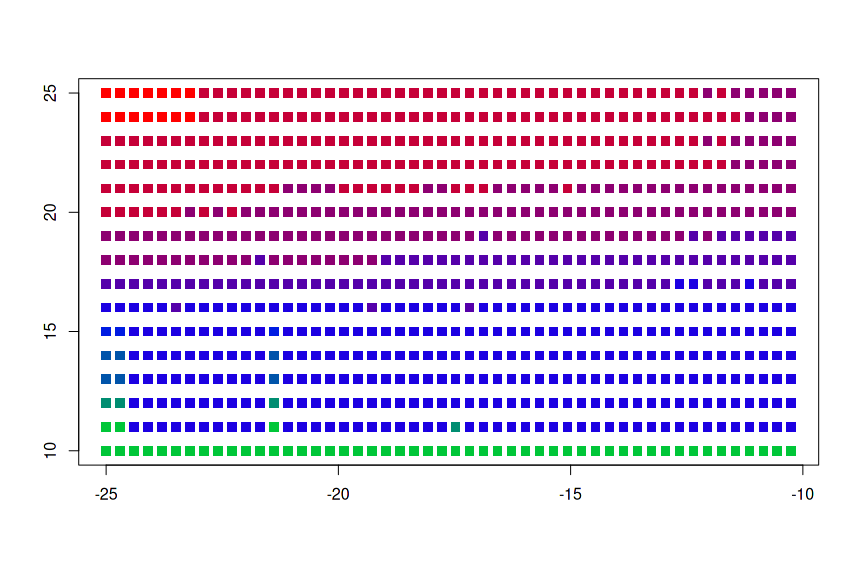
\includegraphics[width=0.95\textwidth]{elegant-gl/datasets/colors_max}
 \end{subfigure}
\end{figure}
\FloatBarrier

\textbf{Vergelijkende screenshots:} hieronder (figuren 8, 9 en 10) staan een aantal paren screenshots van bepaalde (deel)gebieden van het complexe vlak. Elk paar bevat een screenshot van de wortels (rood, op links) en een screenshot van het aantal iteraties per punt in het complexe vlak (blauw, op rechts).
\begin{figure}[!h]
 \caption{Zoom $1.0$, gecentreerd rond $z = 0$}
 \begin{subfigure}{0.49\textwidth}
  
\includegraphics[width=0.9\textwidth]{elegant-gl/scrsh/left_8}
 \end{subfigure}
 \begin{subfigure}{0.49\textwidth}
  
\includegraphics[width=0.9\textwidth]{elegant-gl/scrsh/right_8}
 \end{subfigure}
\end{figure}
\begin{figure}[!h]
 \caption{Zoom $3.13843$, gecentreerd rond $z = \frac{1}{2} + \frac{1}{2}i$}
 \begin{subfigure}{0.49\textwidth}
  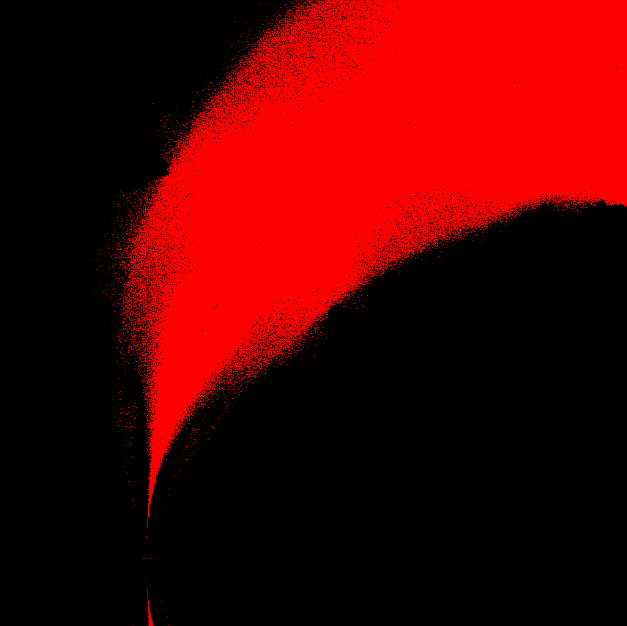
\includegraphics[width=0.9\textwidth]{elegant-gl/scrsh/left_9}
 \end{subfigure}
 \begin{subfigure}{0.49\textwidth}
  
\includegraphics[width=0.9\textwidth]{elegant-gl/scrsh/right_9}
 \end{subfigure}
\end{figure}
\begin{figure}[!h]
 \caption{Zoom $3.7975$, gecentreerd rond $z = -0.0658328 + 0.914028 i$}
 \begin{subfigure}{0.49\textwidth}
  
\includegraphics[width=0.9\textwidth]{elegant-gl/scrsh/left_10}
 \end{subfigure}
 \begin{subfigure}{0.49\textwidth}
  
\includegraphics[width=0.9\textwidth]{elegant-gl/scrsh/right_10}
 \end{subfigure}
\end{figure}

%\FloatBarrier
\newpage

\appendix{}
\section{Testcode Sage}
Deze code werd gebruikt om de Sage-code voor opgave 1.1 (nulpunten van (monische) veeltermen door middel van de companionmatrix) te testen. Voor elke graad van 2 tot en met 10 worden er 10000 (willekeurige) veeltermen van die graad berekend. Het algoritme wordt gebruikt om de nulwaarden te zoeken, waarna de functiewaarden van deze nulwaarden vergeleken wordt met een vaste drempelwaarde (\(1*10^{-15}\))
\begin{lstlisting}[language=Python]
def test_solve(func, poly, margin=1e-15, ring=RDF):
    try:
        sol = func(poly, ring)
    except(ValueError):
        return (True, 0)
    for ans in sol:
        a = abs(poly(ans))
        if a > margin:
            return (False, ans)
    return (True, -1)

def multitest_solve(func, degree=5, samples=10000, margin=1e-15):
    #P.<x> = RDF[]
    P.<x> = RealField(100)[]
    errors = 0
    skipped = 0
    for i in range(samples):
        p = P.random_element(degree)
        (res, err) = test_solve(func, p, margin, RealField(100))
        if res == False:
            errors += 1
        if res == True and err == 0:
            skipped += 1
    print("Ran ", samples - skipped, " tests for polynomials of degree ",
    	degree, "(", skipped, " skipped); ", errors,
    	" solutions outside of margin ", margin)
\end{lstlisting}

\section{Directory-structuur}
Hierbij een kort overzicht van wat waar te vinden is.
\begin{itemize}
 \item \verb|./bruteforce-cuda/|: bevat de code voor de brute-krachtsimplementatie (C++/CUDA implementatie).
 \begin{itemize}
  \item \verb|./bruteforce-cuda/bin/|: wordt gebruikt als output directory voor binaries.
  \item \verb|./bruteforce-cuda/obj/|: wordt gebruikt als objects directory.
  \item \verb|./bruteforce-cuda/src/|: bevat de C++/CUDA source code.
  \item \verb|./bruteforce-cuda/tests/|: bevat de C++/CUDA code voor de tests.
  \item \verb|./bruteforce-cuda/Makefile|: de Makefile om het bruteforce gedeelte eenvoudig te compileren.
 \end{itemize}
 \item \verb|./elegant-gl/|: bevat de code voor de elegantere implementatie (C++/CUDA/OpenGL implementatie).
 \begin{itemize}
  \item \verb|./elegant-gl/bin/|: wordt gebruikt als output directory voor binaries.
  \item \verb|./elegant-gl/datasets/|: bevat een aantal figuren die gebruikt worden in dit document.
  \item \verb|./elegant-gl/glad/|: bevat de GLAD source code (gebruikt om OpenGL te initializeren; gedownload van \href{https://glad.dav1d.de/}{https://glad.dav1d.de/}.
  \item \verb|./elegant-gl/obj/|: wordt gebruikt als objects directory.
  \item \verb|./elegant-gl/scrsh/|: bevat de screenshots voor 2.2.4.
  \item \verb|./elegant-gl/shaders/|: bevat de OpenGL vertex shader en de twee OpenGL fragment shaders.
  \item \verb|./elegant-gl/src/|: bevat de C++/OpenGL source code.
  \begin{itemize}
   \item \verb|./elegant-gl/src/cuda/|: bevat de C++/CUDA source code.
  \end{itemize}
  \item \verb|./elegant-gl/Makefile|: de Makefile om het elegantere gedeelte eenvoudig te compileren
 \end{itemize}
 \item \verb|./figures/|: bevat een deel van de figuren in dit bestand.
 \item \verb|./notebook.ipynb|: het Sage/Jupyter Notebook voor opgave 1.
 \item \verb|./verslag.pdf|: (dit bestand) het verslag.
\end{itemize}

\section{Makefile targets}
Hieronder volgt per Makefile in het project een kort overzicht van elke recept (target) in die Makefile.

\subsection{Bruteforce (./bruteforce-cuda/Makefile)}
\begin{itemize}
 \item \verb|all| (default): compileert en linkt alle code voor \verb|./bruteforce-cuda/bin/bruteforce|; de brute-krachtsimplementatie die alle oplossingen poogt te berekenen.
 \item \verb|cuda|: synoniem voor \verb|all|
 \item \verb|test|: compileert en linkt alle testen, en voert die daarna ook uit.
 \item \verb|clear|: verwijdert alle binaries en/of objecten, en zet daarna de directory structuur klaar voor een volgende compilatie.
\end{itemize}

\subsection{Elegant (./elegant-gl/Makefile)}
\begin{itemize}
 \item \verb|all| (default): compileert en linkt alle code voor \verb|./elegant-gl/bin/gl|; de elegantere implementatie die per pixel probeert een veelterm op te stellen, en daarbij ook het aantal benodigde iteraties weergeeft.
 \item \verb|gl|: synoniem voor \verb|all|.
 \item \verb|cpu|: bouwt een eenvoudige (CPU) implementatie in \verb||. Deze implementatie werd gebruikt voor (de figuren in) 2.2.3.
 \item \verb|clear|: verwijdert alle binaries en/of objecten, en zet daarna de directory structuur klaar voor een volgende compilatie.
\end{itemize}

\end{document}
